% !TeX encoding = UTF-8
% !TeX program = pdflatex
% !BIB program = biber
% LTeX: enabled=false 

\NeedsTeXFormat{LaTeX2e}[2019-10-01]
% **************************************************
% Document Class Definition
% **************************************************
\documentclass[%
    paper=A4,               % paper size --> A4 is default in Germany
    parskip=half,           % spacing value / method for paragraphs
    chapterprefix=false,     % prefix for chapter marksy
    oneside,
    11pt,                   % font size
    headings=normal,        % size of headings
    bibliography=totoc,     % include bib in toc
    listof=totoc,           % include listof entries in toc
    titlepage=off,           % own page for each title page
    captions=tableabove,    % display table captions above the float env
    appendixprefix=false,    % but display a prefix for appendix chapter
    draft=false,            % value for draft version
    % left=2cm,
    % right=18cm,
    % total={6in, 9in}
]{scrreprt}%




% config for titlepage
% !TeX encoding = UTF-8
% !TeX root = MAIN.tex

\newif\ifeng%
%% HINWEISE: Hier müssen folgende Einstellungen vorgenommen werden:
%% PLEASE NOTE: Select your settings here:

%% Sprache: Falls die Dokumentensprache Deutsch ist, \engtrue mit einem %-Zeichen davor auskommentieren:
%% Language: If the document language is German, comment \engtrue with a % sign in front:
\engtrue%

%% Hier den Namen des Autors eingeben:
%% Enter the author’s name here:
\def\author{Philipp Renz}

%% Hier Informationen für den rechten Block unter dem JKU-Logo eingeben, wobei die Elemente mit einem Buchstaben jeweils für die Beschreibung und mit Doppelbuchstaben für den Inhalt sind.
%% Anzuführen bei Masterarbeit: Eingereicht von, Anfegertigt am, BeurteilerIn, Mitbetreuung.
%% Anzuführen bei Dissertation: Eingereicht von, Anfegertigt am, ErstbeurteilerIn, ZweitbeurteilerIn, Mitbetreuung.
%% Anzuführen bei strukturiertem Doktorat: Eingereicht von, Angefertigt am, ErstbetreuerIn, ZweitbetreuerIn, Mitbetreuung.
%%
%% Enter information here for the right block under the JKU logo, whereby the elements should have one letter for the heading and double letters for content.
%% To be given for master thesis: Author, Submission, Thesis Supervisor, Assistant Thesis Supervisor.
%% To be given for doctoral thesis: Author, Submission, First Supervisor, Second Supervisor, Assistant Thesis Supervisor.
\def\elementA{Submitted by}
\def\elementAA{\textbf{\author} \\ 01126686}

\def\elementB{Submitted at}
\def\elementBB{\textbf{Institute for Machine Learning}}

\def\elementC{Thesis Supervisor / First Evaluator}
\def\elementCC{Univ.-Prof.~Mag.~Dr.\@ \textbf{Günter Klambauer}}

\def\elementD{Co-Supervisor}
\def\elementDD{Univ.-Prof. Dr. \textbf{Sepp Hochreiter}}

\def\elementE{Second Evaluator}
\def\elementEE{Prof. Dr. \textbf{Andreas Bender}}

%% Hier Datum eingeben (Monat der Abgabe im Prüfungs- und Anerkennungsservice):
%% Enter the date (Month and year of submission to Examination and Recognition Services):
\def\date{September 2024}

%% Hier Ort eingeben:
%% Enter the location:
\def\place{Linz}

%% Hier Titel eingeben; steht über dem K:
%% Enter the title; it appears above the K:
% \def\title{Advancing Evaluation of Generative Models for Molecules and Deep Learning for Reaction Prediction}
% \def\title{Advancing Molecular Generative Models and Retrosynthesis Prediction: New Evaluation Approaches and Deep Learning Techniques for Drug Discovery}
\def\title{Generative Models in Drug Discovery: \Huge Advancing Assessments, Metrics and Retrosynthesis Prediction}
% \def\title{Advancing Evaluation of Molecule Generators and Deep Learning for Retrosynthesis Prediction}

%% Hier den Typ der Arbeit eingeben (0: Keine Arbeit, 1: Bachelorarbeit, 2: Masterarbeit, 3: Dissertation, 4: Diplomarbeit):
%% Enter the type of paper here (0: Not Thesis, 1: Bachelor’s Thesis, 2: Master’s Thesis, 3: Dissertation, 4: Diploma Degree Thesis):
\def\type{3}

%% Hier ggf. Untertitel eingeben; stehen unter dem K (nur bei 0):
%% If necessary, enter a subtitle here; below the K (only for 0):
\def\subtitle{}

%% Hier den angestrebten akademischen Grad eingeben:
%% Enter the desired academic degree here:
\def\acadDegree{Doktor der Naturwissenschaften}

%% Hier die Studienrichtung eingeben:
%% Enter the major here:
\def\study{Naturwissenschaften}

% Clean thesis data

% !TEX root = my-thesis.tex

% **************************************************
% Files' Character Encoding
% **************************************************
\PassOptionsToPackage{utf8}{inputenc}
\usepackage{inputenc}

% **************************************************
% Load and Configure Packages
% **************************************************
\usepackage[english]{babel} % babel system, adjust the language of the content
\PassOptionsToPackage{% setup clean thesis style
    figuresep=colon,%
    hangfigurecaption=false,%
    hangsection=false,%
    hangsubsection=false,%
    sansserif=false,%
    configurelistings=true,%
    colorize=full,%
    colortheme=bluemagenta,%
    bibfile=references_zotero,%
}{cleanthesis}
\usepackage{cleanthesis}



\hypersetup{% setup the hyperref-package options
    pdftitle={Generative Models in Drug Discovery: Advancing Assessments, Metrics and Retrosynthesis Prediction},    %   - title (PDF meta)
    pdfsubject={Documentation},%   - subject (PDF meta)
    pdfauthor={Philipp renz},    %   - author (PDF meta)
    plainpages=false,           %   -
    colorlinks=false,           %   - colorize links?
    pdfborder={0 0 0},          %   -
    breaklinks=true,            %   - allow line break inside links
    bookmarksnumbered=true,     %
    bookmarksopen=true          %
}



\setcounter{secnumdepth}{3}

\usepackage[utf8]{inputenc}
% \usepackage{scrlayer-scrpage}
\usepackage{scrhack}

% \usepackage[a-1b]{pdfx}[2019-02-27]
\usepackage[T1]{fontenc}
\usepackage{helvet,mathpazo}
\usepackage{microtype}
% \usepackage[english]{babel}
\usepackage[absolute]{textpos}
\usepackage{amsmath,siunitx}
\usepackage[format=plain]{caption}

% \usepackage[onehalfspacing]{setspace}
% \usepackage[section]{placeins} %\FloatBarrier
\usepackage{float} %[H]
\usepackage{enumitem}
\usepackage{subfiles}
\usepackage{cleveref}

% \usepackage[a4paper top=3cm, bottom=3cm, left=0cm, right=2cm, margin=3cm]{geometry} % Adjust margins as needed
\usepackage[margin=3.5cm, bottom=4cm, top=4cm]{geometry} % Adjust margins as needed

\usepackage[
    natbib=true,
    style=authoryear,
    backend=biber,
    maxcitenames=1,
    maxbibnames=99,
    doi=true,
    url=false,
    isbn=false,
    giveninits=true,
    uniquename=false,
    uniquelist=false,
    backref=true,
    date=year,
    ]{biblatex}
\addbibresource{references_zotero.bib}

\AtEveryBibitem{%
    \ifentrytype{inproceedings}{%
        \clearfield{publisher} 
        \clearfield{location}  
        \clearlist{publisher}
    }{}
    % \clearfield{publisher}
    % \clearname{publisher}
    \clearfield{eprintclass} 
    \clearfield{pubstate}
    % \clearfield{eprint}
}

\DeclareNameAlias{sortname}{family-given}

\newcommand{\printpublication}[1]{\AtNextCite{\defcounter{maxnames}{99}}\fullcite{#1}}
\hfuzz=11.002pt 
\usepackage{pdfpages}
\usepackage{blindtext}

\usepackage{acro}
% # load the acronyms package with no italics



\DeclareAcronym{CADD}{
    short = CADD,
    long = computer-aided drug design,
}
\DeclareAcronym{VS}{
    short = VS,
    long = virtual screening,
}
\DeclareAcronym{HTS}{
    short = HTS,
    long = high-throughput screening,
}
\DeclareAcronym{DMTA}{
    short = DMTA,
    long = Design-Make-Test-Analyze,
}
\DeclareAcronym{ML}{
    short = ML,
    long = machine learning,
}
\DeclareAcronym{DL}{
    short = DL,
    long = deep learning,
}
\DeclareAcronym{RNN}{
    short = RNN,
    long = recurrent neural network,
}
\DeclareAcronym{GNN}{
    short = GNN,
    long = graph neural network,
}
\DeclareAcronym{QSPR}{
    short = QSPR,
    long = quantitative structure-property relationship,
}
\DeclareAcronym{QSAR}{
    short = QSAR,
    long = quantitative structure-activity relationship,
}
\DeclareAcronym{DNDD}{
    short = DNDD,
    long = de novo drug design,
}
\DeclareAcronym{NLL}{
    short = NLL,
    long = negative log-likelihood,
}
\DeclareAcronym{VAE}{
    short = VAE,
    long = variational autoencoder,
    first-long-format=\textbf,
}
\DeclareAcronym{LSTM}{
    short = LSTM,
    long = Long Short-Term Memory,
}
\DeclareAcronym{GAN}{
    short = GAN,
    long = Generative Adversarial Network,
    first-long-format=\textbf,
}
\DeclareAcronym{FCD}{
    short = FCD,
    long = Frechet ChemNet Distance,
}

\DeclareAcronym{CASP}{
    short = CASP,
    long = computer-aided synthesis planning,
    % first-long-format=\textbf,
}

\DeclareAcronym{MHN}{
    short = MHN,
    long = modern Hopfield network,
}

\DeclareAcronym{SMILES}{
    short = SMILES,
    long = simplified molecular input line entry system,
}

\DeclareAcronym{ADME}{
    short = ADME,
    long = {absorption, distribution, metabolism, and excretion},
}

\DeclareAcronym{FDA}{
    short = FDA,
    long = Food and Drug Administration,
}

\DeclareAcronym{EMA}{
    short = EMA,
    long = European Medicines Agency,
}

\DeclareAcronym{ELBO}{
    short = ELBO,
    long = evidence lower bound,
}
\DeclareAcronym{SEDiv}{
    short = SEDiv,
    long = sphere exclusion diversity,
}
\usepackage{tocloft}
\setlength{\cftbeforechapskip}{2pt}


\begin{document}
\pagenumbering{roman}			% roman page numbing (invisible for empty page style)
\pagestyle{empty}				% no header or footers
\begin{titlepage}
    \setcounter{page}{0}
    \singlespacing
\sffamily
\small
\setlength{\TPHorizModule}{1mm}
\setlength{\TPVertModule}{1mm}
\mbox{}

\begin{textblock}{97} (142,20)
	\ifeng
		
\includegraphics[width=52mm]{cover/jkuen}
	\else
		
\includegraphics[width=52mm]{cover/jkude}
	\fi
\end{textblock}

\begin{textblock}{85} (155,60)
	\begin{minipage}[t]{40mm}
		\begin{flushleft}
			\ifdefined\elementA%
			{\footnotesize\elementA}
			\vskip.1mm
			\ifdefined\elementAA%
				\elementAA%
			\fi
			\vskip5mm
			\else
			\relax
			\fi
			\ifdefined\elementB%
			{\footnotesize\elementB}
			\vskip.1mm
			\ifdefined\elementBB%
				\elementBB%
			\fi
			\vskip5mm
			\else
			\relax
			\fi
			\ifdefined\elementC%
			{\footnotesize\elementC}
			\vskip.1mm
			\ifdefined\elementCC%
				\elementCC%
			\fi
			\vskip5mm
			\else
			\relax
			\fi
			\ifdefined\elementD%
			{\footnotesize\elementD}
			\vskip.1mm
			\ifdefined\elementDD%
				\elementDD%
			\fi
			\vskip5mm
			\else
			\relax
			\fi
			\ifdefined\elementE%
			{\footnotesize\elementE}
			\vskip.1mm
			\ifdefined\elementEE%
				\elementEE%
			\fi
			\vskip5mm
			\else
			\relax
			\fi
			\date%
		\end{flushleft}
	\end{minipage}
\end{textblock}

\begin{textblock}{85} (155,260)
	\begin{minipage}[t]{40mm}
		{
			\fontfamily{ugq}
			\selectfont
			JOHANNES KEPLER\\
			\ifeng{} UNIVERSITY
			\else UNIVERSITÄT
			\fi
			LINZ\\
		}
		Altenbergerstraße 69\\
		4040 Linz,
		\ifeng{} Austria
		\else Österreich
		\fi \\
		www.jku.at\\
		DVR 0093696
	\end{minipage}
\end{textblock}

\begin{textblock}{165}[0,1](30,140)
	\begin{minipage}[b]{120mm}
		\fontfamily{ugq}
		\fontsize{32pt}{32}
		\selectfont
		\flushleft
		\title
	\end{minipage}
\end{textblock}

\begin{textblock}{120}(30,150)
	
\includegraphics[width=44mm]{cover/arr}
\end{textblock}

\begin{textblock}{165}(30,195)
	\begin{minipage}[t]{120mm}
		\Large
		\ifeng
		\ifcase\type
			\ifdefined\subtitle
				\LARGE
				\subtitle
			\else
				\relax
			\fi
		\or Bachelor Thesis
		\or Master Thesis
		\or Doctoral Thesis
		\or Diploma Thesis
		\fi
		\vskip1mm
		\ifcase\type
			\relax
			\else
			{
				\normalsize to obtain the academic degree of
			}
			\vskip2mm
		\fi
		\ifcase\type
		\relax
		\else
		\acadDegree
		\vskip1mm
		\fi
		{
			\normalsize
			\ifcase\type
				\relax
			\or in the Bachelor's Program
			\or in the Master's Program
			\or in the Doctoral Program
			\or in the Diploma Program
			\fi
		}
		\vskip2mm
		\ifcase\type
			\relax
		\else
			\study
		\fi
		\else
		\ifcase\type
			\ifdefined\subtitle
				\LARGE\subtitle
			\else
				\relax
			\fi
		\or Bachelorarbeit
		\or Masterarbeit
		\or Dissertation
		\or Diplomarbeit%
		\fi
		\vskip1mm
		\ifcase\type%
			\relax
			\else
			{
				\normalsize zur Erlangung des akademischen Grades
			}
			\vskip2mm
		\fi
		\ifcase\type%
			\relax
		\else
			\acadDegree \vskip1mm%
			\fi
			{
				\normalsize
				\ifcase\type%
					\relax
				\or im Bachelorstudium%
				\or im Masterstudium%
				\or im Doktoratsstudium%
				\or im Diplomstudium%
				\fi
			} \vskip2mm
			\ifcase\type% 
				\relax
			\else
				\study%
			\fi
		\fi
	\end{minipage}
\end{textblock}

\end{titlepage}
\clearpage

\pagestyle{plain}				% display just page numbers
% !TeX encoding = UTF-8
% !TeX root = MAIN.tex

{%
\selectlanguage{english}
\chapter*{Abstract}
In recent years the use of generative models in drug discovery has seen a surge, as novel deep
learning architectures have shown great flexibility in generating molecular structures. However, the
evaluation of generative models is challenging and existing benchmarks are often criticized 
for not reflecting the practical utility of the models. In this thesis, we propose new
evaluation metrics and benchmarks for generative models in drug discovery. Another focus of this
work is the application of generative models to retrosynthesis prediction, a crucial task in
computer-aided synthesis planning (CASP). 

The first part of this thesis focuses on observed failure modes in the evaluation of generative
models for de novo molecular design. In particular we show that commonly used metrics used to
evaluate distribution-learning are not sufficient to differentiate complex models from trivial
baseline generators. Secondly, we show how generative models applied to molecular optimization can
overfit to machine learning-based scoring functions, leading to biased evaluations. 

The second part introduces a diversity-based benchmark for goal-directed molecule generators.
Diverse, high-scoring compounds are crucial in drug discovery, as many candidates may fail in later
stages. Previous studies on diverse molecule optimization have been limited by inadequate diversity
measures, non-standardized compute budgets, and lack of model adaptation to diverse optimization settings.
Our benchmark addresses these shortcomings, providing a standardized framework for evaluating
diverse, goal-directed molecule generators and enabling fair model comparisons.

The third part of this thesis focuses on retrosynthesis prediction a crucial task in computer-aided
synthesis planning (CASP). We propose a novel template-based retrosynthesis prediction model based
on Modern Hopfield Networks. Our model takes both the target molecule and the reaction templates 
as input, which allows it to generalize over reaction templates, which improves 
performance, particularly on rare templates. Our model achieves state-of-the-art performance on the USPTO-50k dataset.
while maintaining a significantly lower computational cost compared to existing methods. 

Through our work, we provide insights into the capabilities and limitations of
current generative models for molecules while proposing novel evaluation
strategies. Additionally, our contributions in retrosynthesis prediction enable
more accurate computer-aided synthesis planning. Collectively, these advances
have the potential to accelerate the drug discovery pipeline and facilitate the
development of novel pharmaceutical treatments.
}		% INCLUDE: the abstracts (english and german)
\clearpage
% !TEX root = ../my-thesis.tex
%
\pdfbookmark[0]{Acknowledgement}{Acknowledgements}
\addchap*{Acknowledgement\label{sec:acknowledgement}}

I would like to thank my supervisor, Prof. Dr. Günter Klambauer for his guidance
and support throughout the course of this thesis. I am also grateful to Sepp Hochreiter 
without whom this work would not have been possible. 

I would like to thank my colleagues at the Institute of Machine Learning for
many hours of fruitful discussions and exchange. It was a pleasure being around
you. Especially I would like to thank my co-author Philipp S. It was such a
pleasure collaborating with you, and I'm grateful to have had such a great
colleague to work with. Big thanks also go out to Vihang, Theresa and my
favourite non-co-author Johannes. A big thank you also goes to Birgit and Jenny
who do an awesome job of keeping the institute running, and keeping us all sane.
Herbert and the IT team also deserve a big thank you for keeping our GPUs up and
running.

A special thank you goes to my family for their unconditional support. Thank you 
Alfred, Eveline, Sarah, and Wolfgang, Ronja, Raphi for always being there for me. 

Finally, I would like to all my friends for their support and for just being
there. This includes the kayakers, acro people, and the legendary PL crew
(including the ones who would not call it that.). You're al-rye-ght. Life would
not as rich without you. Special thanks go out to Alex and Alina. I'm lucky to
have you as friends. 

Last but not least, I would like to thank my partner, Jordan. Although you only 
joined me for the last part of this journey, you have been a constant source of
support and love. I'm grateful to have you in my life.

 % INCLUDE: acknowledgement
\clearpage
% 
\currentpdfbookmark{\contentsname}{toc}
\setcounter{tocdepth}{3}		% define depth of toc
\vspace{-3cm}
\tableofcontents				% display table of contents
% 
% \printacronyms[name=List of Acronyms,heading=chapter*,display=used,sort=true]
\acsetup{
    make-links = true , % boolean
    format = \textup, % standard
    list / local, % boolean option of the list module
    list / display = all, % choice option of the list module
    format/first-long = \textup,
    format/long = \textup,
    format/short = \textup,
    format/alt = \textup,
}


% --------------------------
% Body matter
% --------------------------
\pagenumbering{arabic}			% arabic page numbering
\setcounter{page}{1}			% set page counter
\pagestyle{scrheadings}			% header and footer style

\chapter{Introduction\label{chap:introduction}}
% Drug discovery is important. 
Drug discovery is the process of identifying new medicines and bringing them to
market. The discovery of novel pharmaceutical treatments has been a major driver
of quality of life over the centuries. While discovery of new drugs has started 
in serendipitous and lucky discoveries, advances in science and technology  
allowed for a more systematic and data-driven approach over the last decades. 

% Traditional way of finding candidates.
One of the key challenges of the drug discovery process is the identification
of novel promising drug candidates. The efficacy of a drug is usually determined by its ability
to interact with a biological target in the body. To find such molecules,
the traditional approach is to synthesize and test the molecules efficacy first in laboratory
experiments, and finally in clinical studies. However, this process is usually very expensive, time-consuming
and can involve risks for patients.

% Computer aided drug discovery
Computer aided drug discovery (CADD) aims to accelerate the drug discovery
process by using computational methods. Applications range from basic chemical
information processing, over physical simulation of molecular interactions, to
sophisticated machine learning methods. Advances in deep learning
\citep{chenRiseDeepLearning2018} have led to breakthroughs in many different
areas of drug discovery, including highly accurate protein structure prediction 
achieved by AlphaFold \citep{todo}, chemical property prediction
\citep{mayrDeepToxToxicityPrediction2016,todo}, synthesis planning
\citep{seglerNeuralSymbolicMachineLearning2017} and molecule generation
\citep{todo}. These advances help by reducing the need for expensive 
wet-lab experiments and can assist chemists in drug design tasks. 

% Significance and objectives of the thesis
In this thesis, we focus on two key areas where machine learning can help to
accelerate the drug discovery process: generative models for molecules and
computer-aided synthesis planning (CASP). Generative models have been shown to
be able to efficiently find molecular structures satisfying property profiles of
interest, and have been used to generate novel drug candidates. However, the
evaluation of generative models is challenging, as the outputs of these models
are usually complex, structured objects, and there are often no straightforward
ways to evaluate the quality or relevance of the generated molecules. In this
thesis, we address this issue by proposing new evaluation metrics and benchmarks
for generative models.

% CASP
Computer-aided synthesis planning (CASP) assists chemists in the task of
synthesizing target molecules. CASP tools are based on a combination of planning
algorithms and computational chemical reaction models, and suggest synthesis
plans for molecules of interest. Highly accurate chemical reaction models are
necessary for satisfactory performance of CASP tools. Many such models are based
on reaction templates, which encode the connectivity changes between atoms that
occur during a chemical reaction. In this thesis we propose a novel
template-based reaction model for the problem of single-step retrosynthesis
prediction \citep{todo}. 

% PROMISE
This thesis is structured as follows. In \cref{sec:generative-models} we give 
an overview of generative models for molecules, discuss the challenges of evaluating
these models and present our contributions to this field. In \cref{sec:retrosynthesis}
we give a short overview of computer-aided synthesis planning and outline our contributions. 
\Cref{sec:publications} lists the publications that are part of this thesis and 
related publications. \Cref{chap:publications} reprints the publications
and their corresponding supplementary material. Finally, \cref{chap:conclusion} concludes
the thesis and gives an outlook on future work.



% \begin{minipage}
% : Rational drug discovery.
% This approach starts with the identification of a biological target in the body 
% which is hypothesized to be associated with a disease phenotype. 
% One then attempts to find a small molecule that can change the activity of 
% the target in the desired way. While this way of searching for new drugs 
% is more direct than phenotypic drug discovery the identification of 
% drug targets can be challenging and given the complex interconnectedness 
% of biochemical pathways, it is not fully understood how some drugs work, 
% which goes even for highly popular ones.

% Phenotypic drug discovery takes this trial-and-error approach and applies it 
% in a systematic manner. The focus in this approach, which is also called forward 
% pharmacology, lies on screening collections of small molecules or other potential 
% medicines for pharmaceutical effects. Once a pharmacologically active molecule 
% has been found the aim is to discover how to use it's effect therapeutically. 
% This process can proceed without knowing the biochemical mode of action, of how 
% a drug actually achieves its effect. 

% How were new medicines discovered?
% David C. Swinney & Jason Anthony 
% Lots of molecules also by phenotypic screening

% One of core goals in both approaches is to find molecules with a desired
% pharmacological profile, which includes primarily the ability of a molecule to
% modify a target, but also other important
% properties, e.g. absorption, distribution, metabolism, excretion or toxicity. 
% To find such molecules, specially designed wet-lab experiments called \emph{assays} 
% are usually use to measure these properties of interest. The number of tested 
% molecules can range from numbers in the tens to millions of tested molecules
% in high-througput screening. 

% \emph{Computer-aided drug design} aims to reduce the need 
% for these expensive experiments using computational methods. 
% The field of quantitative structure activity/property relationship (QSAR/QSPR)
% aims to find an accurate computational model of the drug-target interaction. 
% Structure-based methods make use of the known structures of the drug and target 
% and calculate binding affinity using physical modelling. 
% In contrast, ligand-based methods find links between molecular structures
% and measured experimental outcomes. In recent years, machine learning methods 
% have shown great promise at modelling these relationships. 
% Using these models one can prioritize which of the molecules available in a screening 
% collection to test next, to avoid wasting ressources on unpromising compounds.

% However, this approach of virtual screening is limited to existing screening collections
% and computational constraints. The $~10^{12}$ \citep{todo} molecules that can be realistically 
% evaluated fall far short of the $10^{23}$-$10^{60}$ drug-like molecules 
% which are estimated to exist \citep{todo}, and necessarily miss out on promising drug candidates.
% Generative models aim to alleviate this problem, by using the QSAR/QSPR function as a guiding signal 
% in order to be able to explore chemical space in a goal-directed manner. 
% The evaluation 

% However, the process of bringing a new drug to market is a long, expensive, and risky endeavor.
% Estimates of bringing a new drug to market range between 2.6 and xxx 
% billion USD \citep{todo}. When successful, however, a new drug can be a major source of
% relief for patients.

% % Traditional way of finding candidates.
% One of the key challenges of the drug discovery process is the identification
% of novel promising drug candidates. Traditionally, this is done by synthesizing
% and testing the molecules efficacy in a laboratory and clinical studies. 
% However, this process is usually very expensive, time-consuming and can be risky for 
% patients. 

% % ML can help to find promising candidates
% Machine learning (ML) and deep learning (DL) have the potential to accelerate
% the drug discovery process. Recent advances in ML, especially in the subfield of deep learning
% have led to a surge in interest in applying ML and DL to drug discovery, 
% culminating in breakthroughs such as AlphaFold \citep{todo}. 
% In this thesis, we focus on two key areas where ML and DL can help to accelerate
% the drug discovery process: generative models for molecules and computer-aided
% synthesis planning (CASP).
% \end{minipage}

\section{Advancing the Evaluation of Generative Models for Molecules\label{sec:generative-models}}
% Generative models help to find promising candidates
Goal-directed molecule generators aim to address the challenge of finding novel
molecular structures satisfying a property profile of interest. These property
profiles can include a range of properties, including the activity against a
target, or other important traits such as solubility or toxicity. Given a
computational scoring function that encodes the relevant properties, generative
models operate in a feedback loop, where the scoring function guides the
generation of molecular structures. This contrasts with the traditional approach
of virtual screening \citep{todo}, where a fixed virtual library of molecules is
searched in a brute-force manner. This simple way of searching the chemical
space is inefficient and is not able to tap into the possibilities provided by
the vastness of drug-like chemical space, which is estimated to contain between
$10^{23}$-$10^{60}$ molecules. Generative models, on the other hand, hold the
promise of being able to search chemical space more efficiently and come up with
promising drug candidates.

Triggered by advances in deep learning, the field of generative models for
molecules has seen a surge in interest in recent years. The first deep-learning
based generative models for molecules were based on recurrent neural networks
(RNNs) originally proposed for text generation. After this early work by
\citep{seglerGeneratingFocusedMolecule2018} and
\citep{gomez-bombarelliAutomaticChemicalDesign2018} a great number of different
models have been published
\citep{eltonDeepLearningMolecular2019,sanchez-lengelingInverseMolecularDesign2018}.
These models are based on a large variety of architectures and training
strategies, including autoregressive models, generative adversarial networks
(GANs), variational autoencoders (VAEs), flow-based models
\citep{madhawaGraphNVPInvertibleFlow2019}. One key design choice is the
representation of the molecules, which can be based on SMILES strings,
graph-based representations or 3D structures
\citep{eltonDeepLearningMolecular2019,sanchez-lengelingInverseMolecularDesign2018,pangDeepGenerativeModels2024}.

Generative models are often divided into two categories: \emph{goal-directed}
and \emph{distribution-learning} models. Distribution-learning models learn
general structural patterns in molecules and aim to sample novel molecules that
the training data in distribution. These models are then most often used as a
base for goal-directed models, which aim to find molecules that satisfy a
property profile of interest. These properties are usually encoded in a
scoring function, which is then used to guide the generation process, in a
reinforcement learning style feedback loop.

% The evaluation of generative models is challenging. 
While generative models have shown great promise in generating stable chemical
structures their evaluation is often challenging. While evaluation in
discriminative tasks is usually a straightforward evaluation on a hold-out test
set, the evaluation of generative models requires more complex evaluation
schemes and require to take into account various aspects of the generated
molecules. This has led to the development of a range of evaluation metrics
\citep{preuerFrechetChemNetDistance2018,gaoSynthesizabilityMoleculesProposed2020}
and benchmarks for generative models
\citep{polykovskiyMolecularSetsMOSES2020,brownGuacaMolBenchmarkingModels2019}.
However, the evaluation of generative models is still an active area of research
and challenges remain. In this thesis, we address some of these challenges which
are outlined in the following sections.

\subsection{Evaluation of Distribution-Learning Models}
The evaluation of distribution-learning methods has posed challenges in
different applications, apart from the generation of molecules. While so called
\emph{likelihood-based} models, such as autoregressive models or flow-based
models, can be evaluated using metrics like the negative log-likelihood or
perplexity evaluated on a hold-out test set, other models such as generative
adversarial networks (GANs) \citep{goodfellowGenerativeAdversarialNetworks2014}
do not offer the possibility of this a straightforward evaluation. To this end
alternative metrics have been proposed, spawning its own subfield of research
\citep{heuselGANsTrainedTwo2017}.

In the field of cheminformatics new metrics have been proposed to evaluate the
quality of generated molecules and how well they match the training data in
distribution \citep{preuerFrechetChemNetDistance2018}.
\citet{polykovskiyMolecularSetsMOSES2020} and
\citet{brownGuacaMolBenchmarkingModels2019} introduced the Moses and GuacaMol
benchmarks respectively, which evaluate the quality of generated molecules using
a combination of metrics. Among these are the FCD metric
\citep{preuerFrechetChemNetDistance2018}, the internal diversity
\citep{benhendaChemGANChallengeDrug2017} of the generated molecules, or the
KL-divergence between the distributions of chemico-physical properties of the
generated molecules and the training data.

It is however not clear how informative these metrics actually are and how well
they correlate with the actual usefulness of the tested generative models. In
\citep{renzFailureModesMolecule2019} (\cref{sec:failure-modes}) we show the
limitations of the GuacaMol distribution-learning benchmark, by evaluating the
performance of different sophisticated generative models on this benchmark, and
comparing it to a simple baseline model that generates molecules by introducing
minor variations of the molecules in the training data. We show that the 
most of the tested generative models do not outperform the simple baseline
model, or only do so marginally. This suggests that the tested benchmarks
are not be able to distinguish state-of-the-art generative models 
from simple baseline models, and call for a more comprehensive evaluation of
distribution-learning models. \Cref{sec:failure-modes} reprints
the corresponding publication.

\subsection{Overfitting to Scoring Functions Biases in Goal-Directed Generation}
In goal-directed generation tasks, the generative models are tasked to find
molecules with high scores according to a scoring function that encodes the
desired properties of the generated molecules. The scoring functions used in
these tasks are often based on ML models trained on experimental
data. This can lead to problems, as the optimization process can overfit to
biases of these ML models. 

It is a well-known problem in generative modelling that the optimizing the
output of classification/regression models with respect to their inputs can lead
to unsatisfactory results \citep{todo}. In the context of goal-directed molecule
generators we identified two possible failure modes: Firstly, the generative
models can overfit to artifacts of the scoring function, which are not actually
relevant for the properties of interest. Secondly, the generative models may
overfit to the training samples used to train the scoring function, which can
lead to a lack of novelty in the generated molecules.

In \citep{renzFailureModesMolecule2019} we introduce \emph{control scores} that
give information whether the optimization overfits to artifacts of the scoring
functions, or the training data. We do this by training additional scoring
functions, trained with either a different random initialization or trained on a
hold-out subset of the the available training data. Using this approach, we can
show that generative models overfit to the scoring function's random
initialization and to high-scoring training samples. This shows that the reported
performance of these models is an overestimation, and that our control 
scores can be used to obtain a more meaningful evaluation of goal-directed 
molecule generators. \Cref{sec:failure-modes} reprints
the corresponding publication.

\subsection{Diversity-based benchmarking of Goal-Directed Generators\label{sec:divopt}}
% Why is diversity important?
The diversity of the generated molecules is an important aspect in the
application of goal-directed generative models. Given that the scoring functions
are usually only an imperfect and incomplete approximation of the desired
properties, finding a diverse set of molecules that score well can increase the
success chancess of downstream stages of the drug discovery project. Given the
expected failure of some of the candidates in later experiments, having a backup
of other candidates with somewhat different structure can be beneficial.

It is unclear how well current generative models perform in generating diverse
high-scoring molecules, which is due to a combination of two main factors. 
Firstly, many commonly used diversity metrics are inadequate for evaluating
diverse optimization approaches. This results in uninformative benchmarks that
do not meaningfully measure the diversity of the generated molecules. Secondly,
a meaningful comparison of goal-directed generators necessitates a standardized
compute budget. This is because the performance of generative models depends strongly 
on the amount of ressources available for training and evaluation.

In \citep{renzBenchmarkingEfficiencyGenerative2024} we introduce a benchmark for
diverse optimization that addresses the above-mentioned issues. In this
benchmark, we evaluate the diversity of the generated molecules using a recently
proposed diversity metric \#Circles \citep{xieHowMuchSpace2023}. We compare the
performance of diverse optimization approaches under two different compute
budgets, namely a fixed number of scoring function evaluations and a fixed time
budget. The first setting is relevant for applications where the cost of
evaluating the scoring function dominates the optimization process, while the
second setting is relevant for scoring functions that are cheap to evaluate.
Using this setup we test 14 goal-directed optimization methods and show how
SMILES-based auto-regressive models dominate the benchmark.
\Cref{sec:diverse-efficiency} reprints the corresponding publication.

\section{Retrosynthesis Prediction\label{sec:retrosynthesis}}
% Retrosynthesis planning is important and ML can help
Drug candidates, whether suggested by generative models or found by other means,
at some point need to be synthesized in for further testing and 
eventually for use in patients. The synthesis of a molecule is usually a complex
process, involving multiple steps of chemical reactions. Computer-aided synthesis 
planning (CASP) can help by finding new synthesis routes for a target molecule.
In some cases, this can lead to more efficient and cheaper synthesis routes, or
even enables the synthesis of previously inaccessible molecules.

% Synthesis planning 
The most popular approach to CASP is retrosynthesis planning. Starting from a
target molecule, the goal is to predict a chain of chemical reactions that can
transform readily available starting materials into the target molecule. This
problem is usually formulated as a graph search problem, where the nodes are
molecules and the edges are chemical reactions. The goal is to find a path from
the target molecule to a set of starting materials, which can be synthesized in
the laboratory. The connectivity of this graph is given by retrosynthesis
prediction models, which given a target product, predict which reactants it can
be made from. Highly accurate retrosynthesis prediction models are necessary for
the success of CASP tools, as otherwise the suggested synthesis routes might not
be feasible in the laboratory.

% A prominent approach to CASP is template-based planning
% Mention transformers and graph-based models
Template-based models are a popular approach to retrosynthesis prediction. These
models use so called reaction templates, which are graph transformation rules 
that encode connectivity changes between atoms during a chemical reaction. These 
templates can be either automatically extracted from a reaction database or
hand-coded by a chemist. Given a target molecule, the goal is then reframed as a
classification task, where the model predicts which templates can be used to
synthesize the target. Application of the graph transformation rules then leads
to reactants that can be used to synthesize the target molecule. While popular, 
these models have some limitations, in common datasets many templates only occur 
in few training samples, which makes it difficult to train a model that generalizes
well for these rare templates.

In \citep{seidlImprovingFewZeroShot2022} we study the problem of single-step
retrosynthesis prediction. Given a target molecule, the goal is to predict a
set of reactants that can be used to synthesize the target molecule.
Template-based models are a popular approach to single-step retrosynthesis
prediction. These models use so called reaction templates, which are
either extracted from a reaction database or hand-coded by a chemist.
Given a target molecule, the goal is then reframed as a classification task,
where the model predicts which templates can be used to synthesize the target.

In \citep{seidlImprovingFewZeroShot2022} we propose a novel approach to
template-based retrosynthesis prediction. We use a multimodal learning approach
that learns to associate relevant templates to product molecules using a Modern
Hopfield Network \citep{ramsauerHopfieldNetworksAll2020}. Our model can leverage
structural information about the templates and can make use of similarities
between them. This allows for improved generalization, especially for templates
with few training samples and even for unseen templates. This model is several
times faster than comparable methods and shows good predictive performance.
\Cref{sec:mhn-react} reprints the corresponding publication.

\section{List of Publications\label{sec:publications}}
This thesis comprises the work published in the following papers:

\begin{itemize}
    \item \fullcite{renzFailureModesMolecule2019}
    \item \fullcite{renzBenchmarkingEfficiencyGenerative2024}
    \item \fullcite{seidlImprovingFewZeroShot2022}
\end{itemize}

% give overview over my other publications
\paragraph{Other Publications} Besides the papers listed above, I have also
contributed to the following publications:

\begin{itemize}
    \item \fullcite{preuerFrechetChemNetDistance2018}
    \item \fullcite{renzUncertaintyEstimationMethods2019}
    \item \fullcite{hofmarcherLargescaleLigandbasedVirtual2020}
    \item \fullcite{renzLowCountTimeSeries2023}
\end{itemize}
% \def\skippdf{1}

\chapter{Publications\label{chap:publications}} % noqa

This chapter reprints the papers comprising this thesis as originally published. The licences are
listed in the respective chapters and the copyright is held by the respective authors. In order to fit the
document dimensions, reprinted publications may be scaled in size and/or cropped.

\clearpage
\thispagestyle{plain}
\section{On Failure Modes in Molecule Generation and Optimization\label{sec:failure-modes}}
This publication is reprinted under a \href{https://creativecommons.org/licenses/by-nc-nd/4.0/}{CC BY-NC-ND} license.
\ifx\skippdf\undefined
    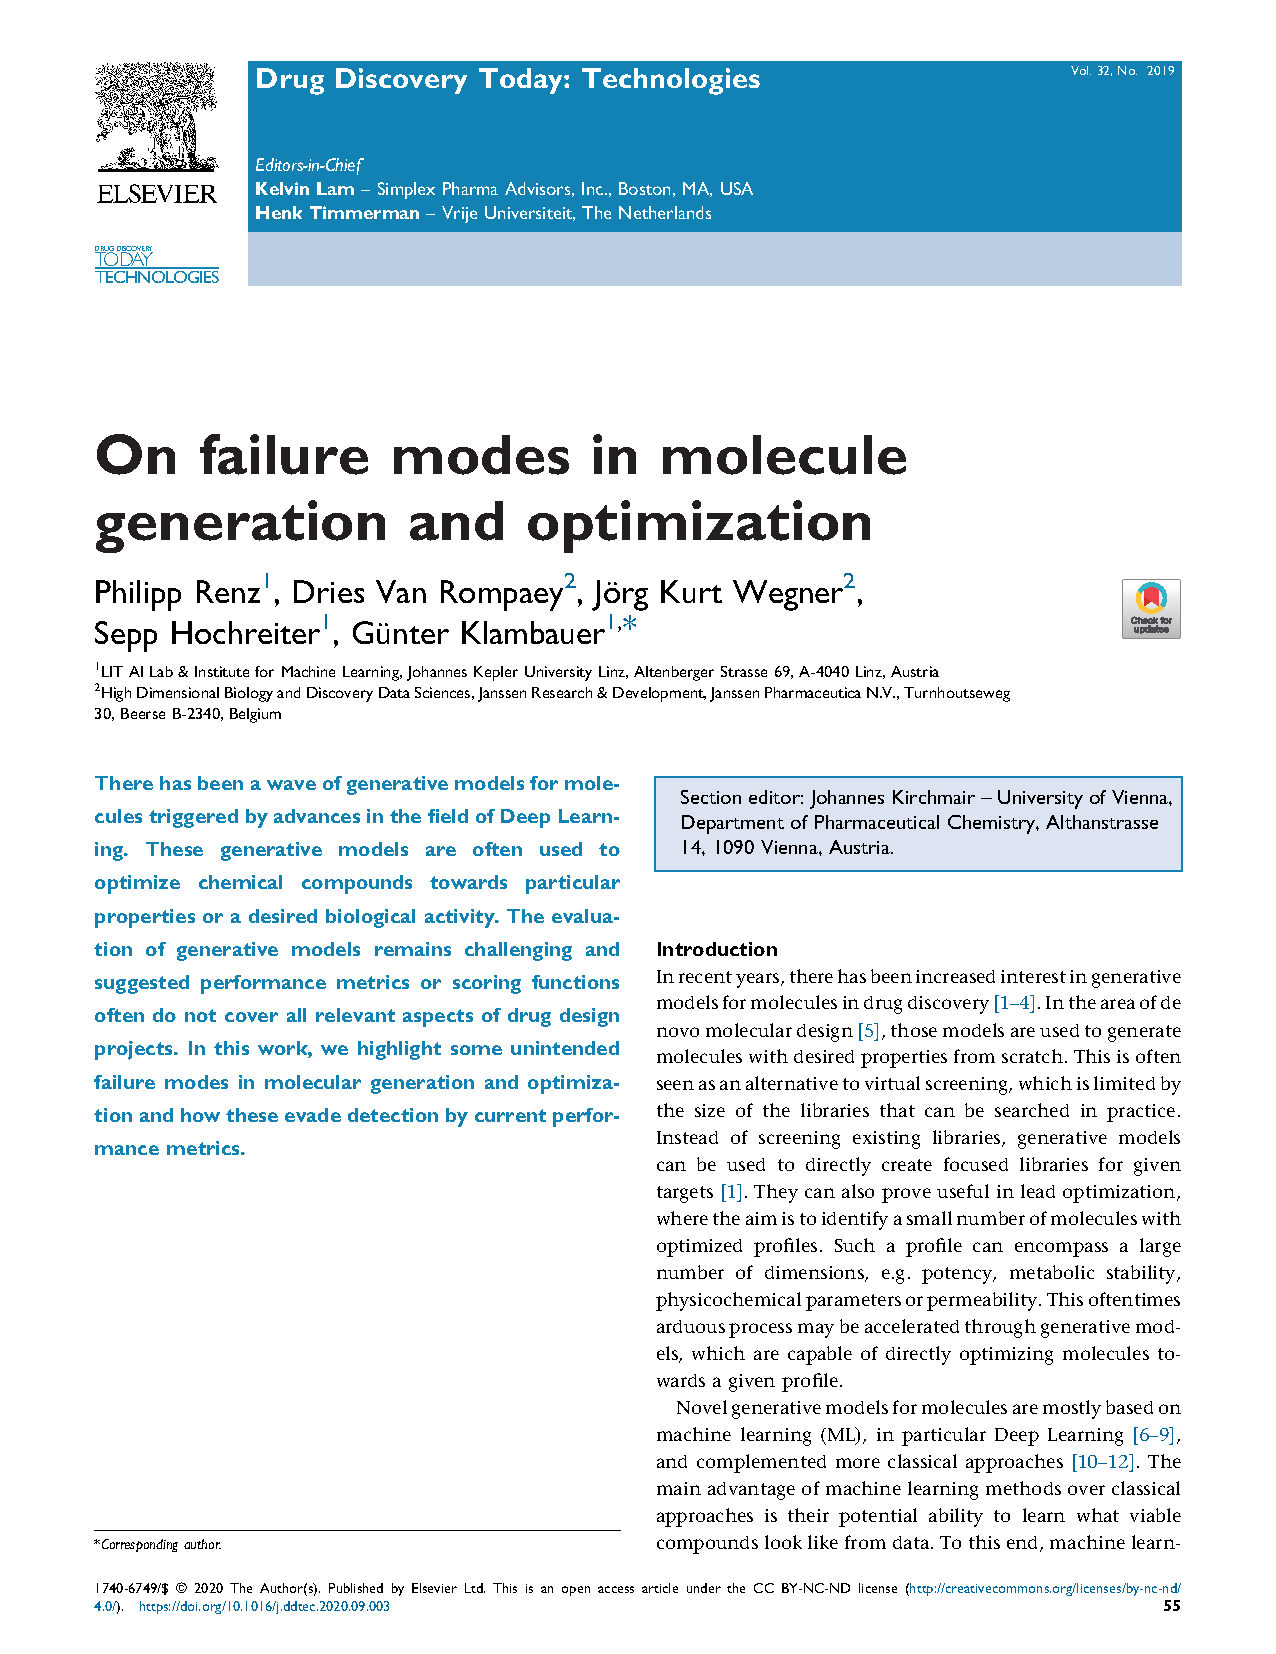
\includepdf[
        pages=-,
        frame,
        width=1.1\linewidth,
        pagecommand={\thispagestyle{scrheadings}},
        offset=0cm 0.9cm,
        trim=0.5cm 0.1cm 0.5cm 0.1cm,
    ]{papers/failure-modes.pdf}
    \includepdf[
        pages=-,
        frame,
        % height=\textheight,
        width=1.1\linewidth,
        pagecommand={\thispagestyle{scrheadings}},
        offset=0.0cm 0.9cm,
        trim=2.1cm 1.5cm 2.1cm 2cm,
    ]{papers/failure-modes-si-recompiled.pdf}
\fi


\clearpage
\thispagestyle{plain}
\section{Diverse Hits in De Novo Molecule Design: Diversity-Based Comparison of Goal-Directed Generators\label{sec:diverse-hits}}
This publication is reprinted under a \href{https://creativecommons.org/licenses/by/4.0/}{CC BY 4.0} license.

\ifx\skippdf\undefined
    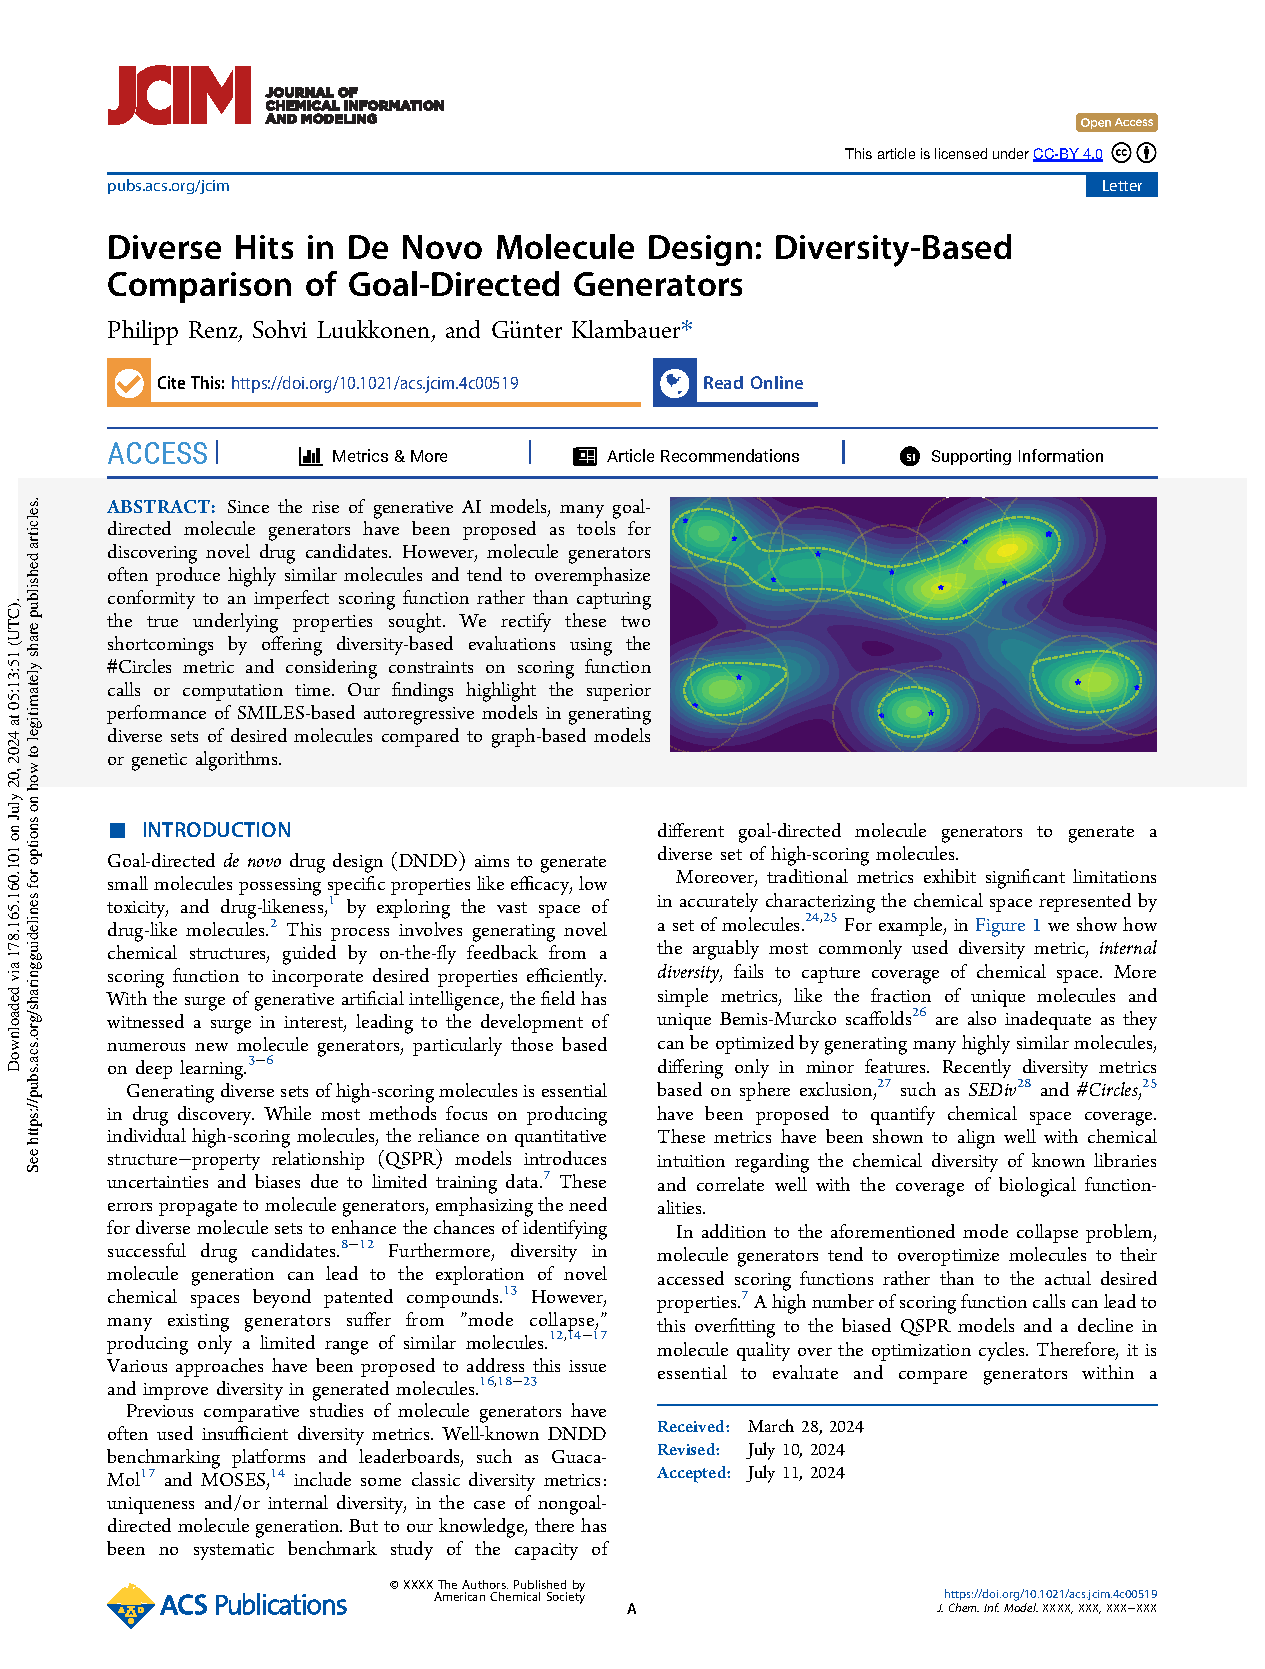
\includepdf[
        pages=-,
        frame,
        width=1.1\linewidth,
        % height=\textheight,
        pagecommand={\thispagestyle{scrheadings}},
        offset=0.0cm 0.9cm,
        trim=0cm 0.0cm 0cm 0.0cm,
    ]{papers/diverse-hits.pdf}

    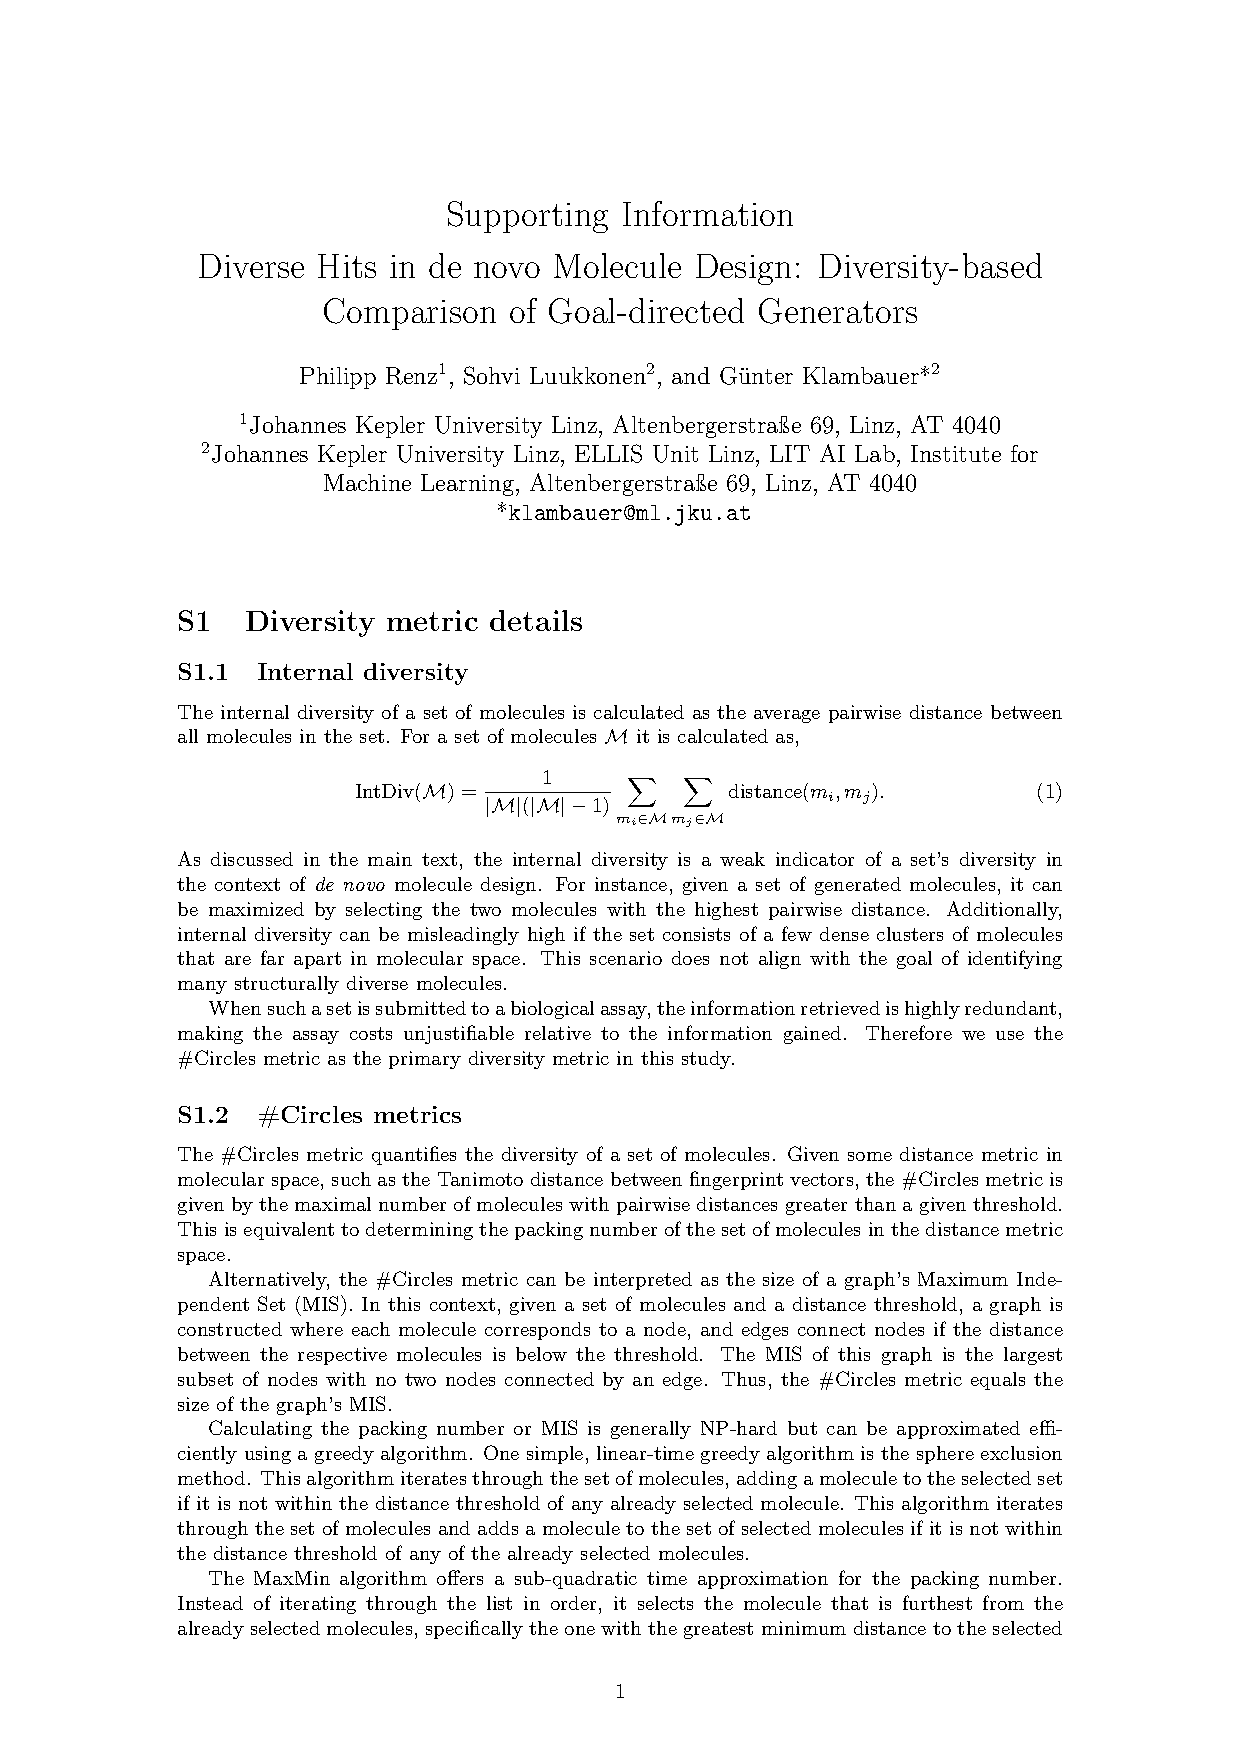
\includepdf[
        pages=-,
        frame,
        width=1.1\linewidth,
        % height=\textheight,
        pagecommand={\thispagestyle{scrheadings}},
        offset=0.0cm 0.8cm,
        trim=1cm 0.5cm 1cm 0.5cm,
    ]{papers/diverse-hits-si.pdf}
\fi


\clearpage
\thispagestyle{plain}
\section{Improving Few- and Zero-Shot Reaction Template Prediction Using
  Modern Hopfield Networks\label{sec:mhn-react}}

This publication is reprinted under a \href{https://creativecommons.org/licenses/by/4.0/}{CC BY 4.0} license.

\ifx\skippdf\undefined
    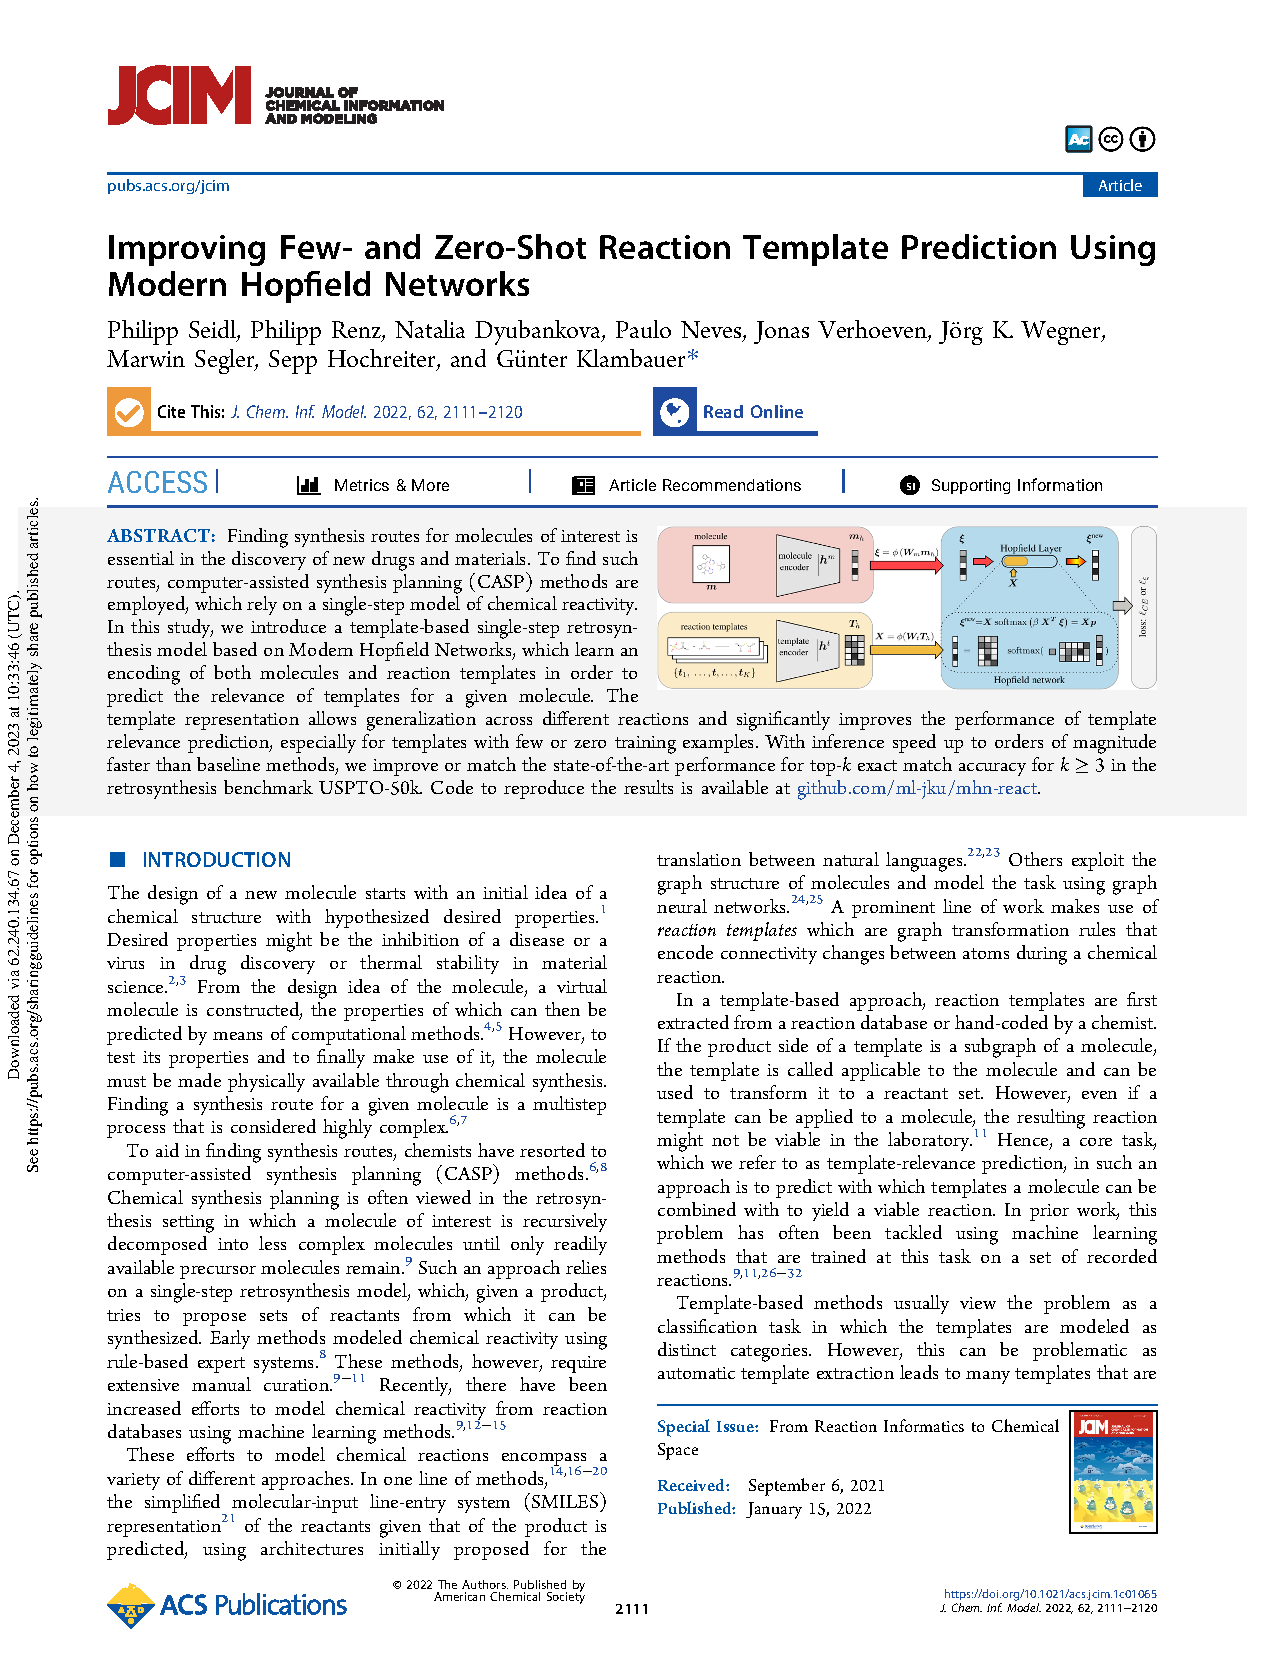
\includepdf[
        pages=-,
        frame,
        width=1.1\linewidth,
        % height=\textheight,
        pagecommand={\thispagestyle{scrheadings}},
        offset=0.0cm 0.9cm,
        trim=0cm 0.0cm 0cm 0.0cm,
    ]{papers/mhn-react.pdf}

    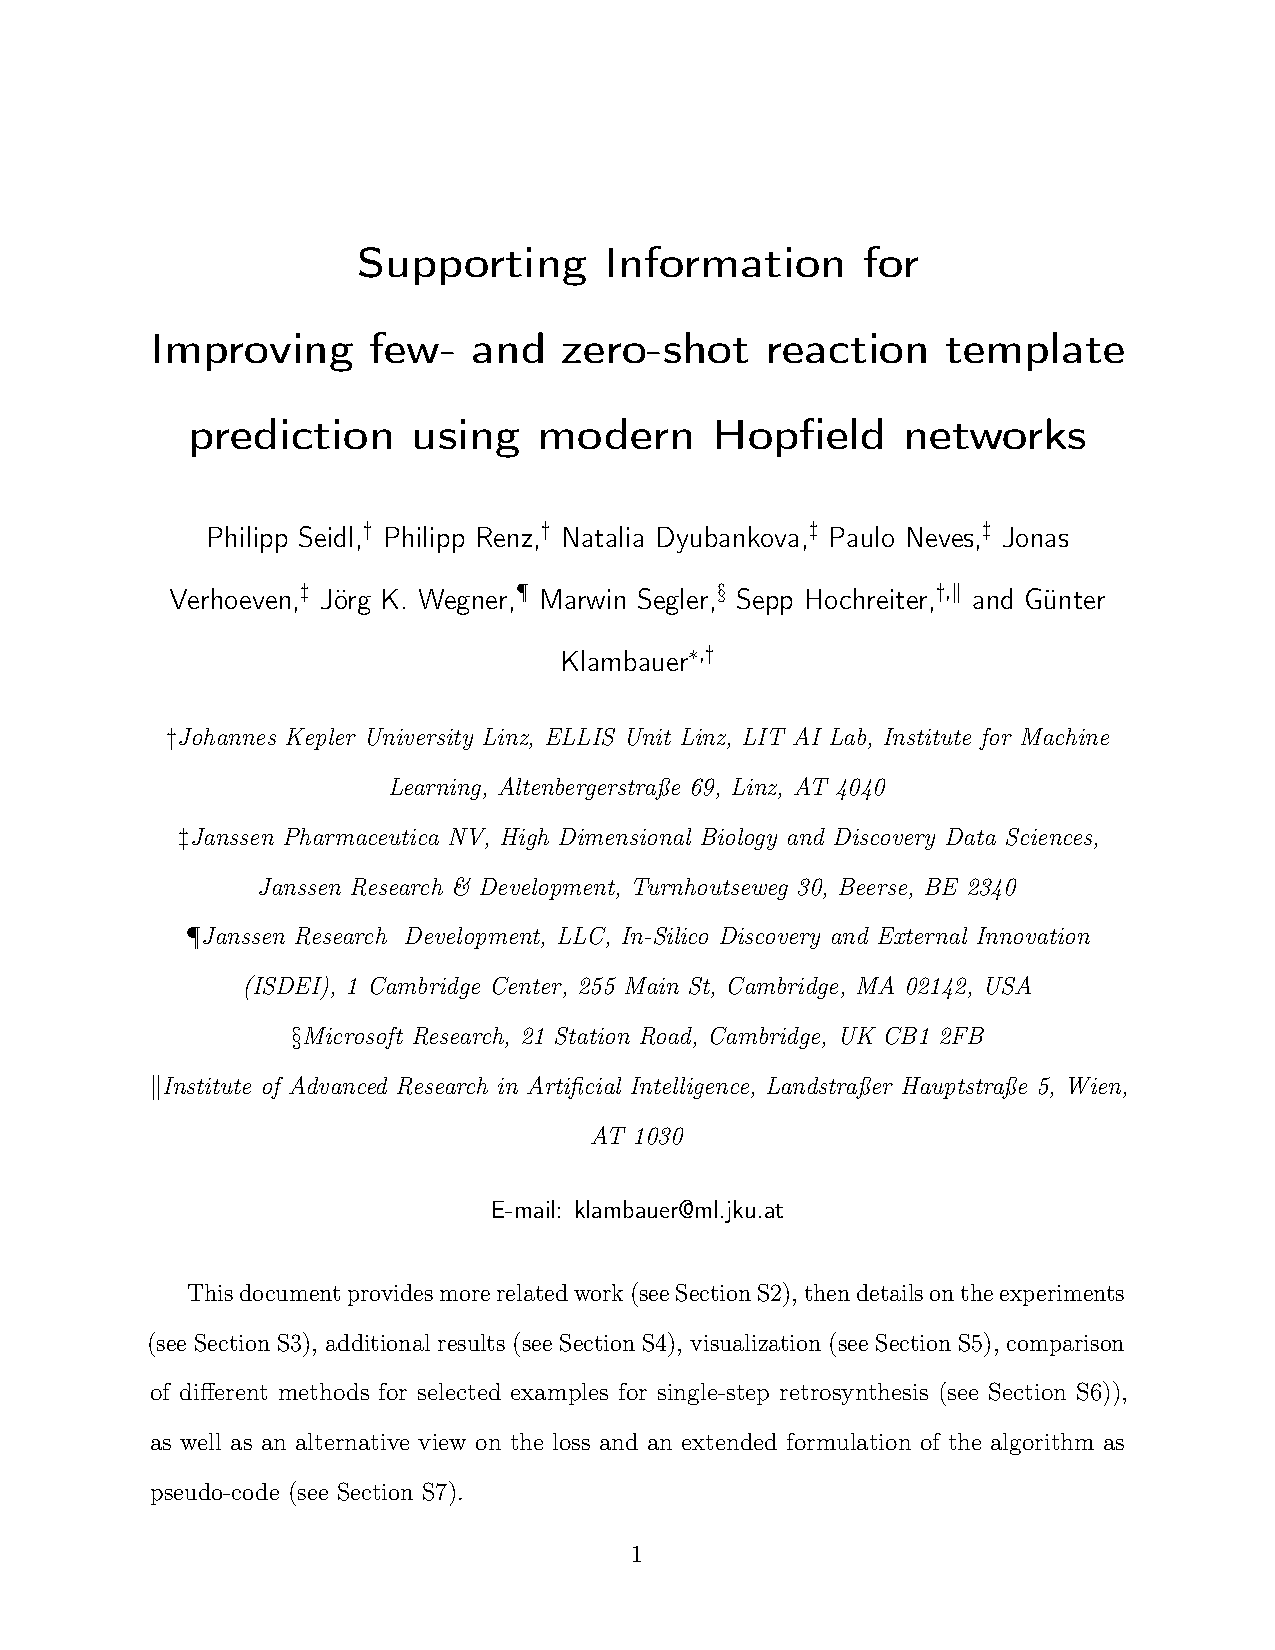
\includepdf[
        pages=-,
        frame,
        width=1.1\linewidth,
        % height=\textheight,
        pagecommand={\thispagestyle{scrheadings}},
        offset=0.0cm 0.8cm,
        trim=1cm 0.5cm 1cm 0.5cm,
    ]{papers/mhn-react-si.pdf}
\fi


\chapter{Conclusion and Outlook\label{chap:conclusion}}
The work in this thesis has focused on
advancing the application of generative models in drug discovery, concentrating on two main aspects:
Firstly, we identified limitations in the evaluation of generative models for de novo molecular
design, and proposed ways to make evaluation more informative and relevant to practical
applications. Secondly we introduced a novel template-based model for retrosynthesis prediction
that matches or exceeds the performance of existing methods, performing particularly well on rare
reaction templates.

In the first part of this thesis, we showed how established ways of evaluating distribution-learning
models cannot differentiate complex models from trivial baseline generators. We also showed
how goal-directed generative models used to optimize scoring functions can be biased towards the
scoring function, leading to overfitting and biases to already known high scoring molecules contained
in the training data.

The second part of this thesis introduced a diversity-based benchmark for goal-directed molecule
generators. This benchmark addresses the shortcomings of previous benchmarks by adressing the issues
of inadequate diversity measures, non-standardized compute budgets, and lack of model adaptation to
the diverse optimization setting. We used this benchmark to evaluate a range of generative models
comparing them in a meaningful way.

The last part of this thesis introduced a novel template-based model for retrosynthesis prediction
based on Modern Hopfield Networks. This model leverages a
multi-modal approach that combines reaction templates and target molecules. Our model is able to
generalize over reaction templates and performs particularly well on rare templates. We showed that
our model matches or exceeds the performance.

In conclusion, our work provides insights into the capabilities and limitations of current generative
models for molecules and proposes novel evaluation strategies. Additionally, our contributions in
retrosynthesis prediction enable more accurate computer-aided synthesis planning.
We hope that our work will help to accelerate the drug discovery pipeline and facilitate the development
of novel pharmaceutical treatments.
\appendix
\chapter{Curriculum Vitae}

% \ifx\skippdf\undefined
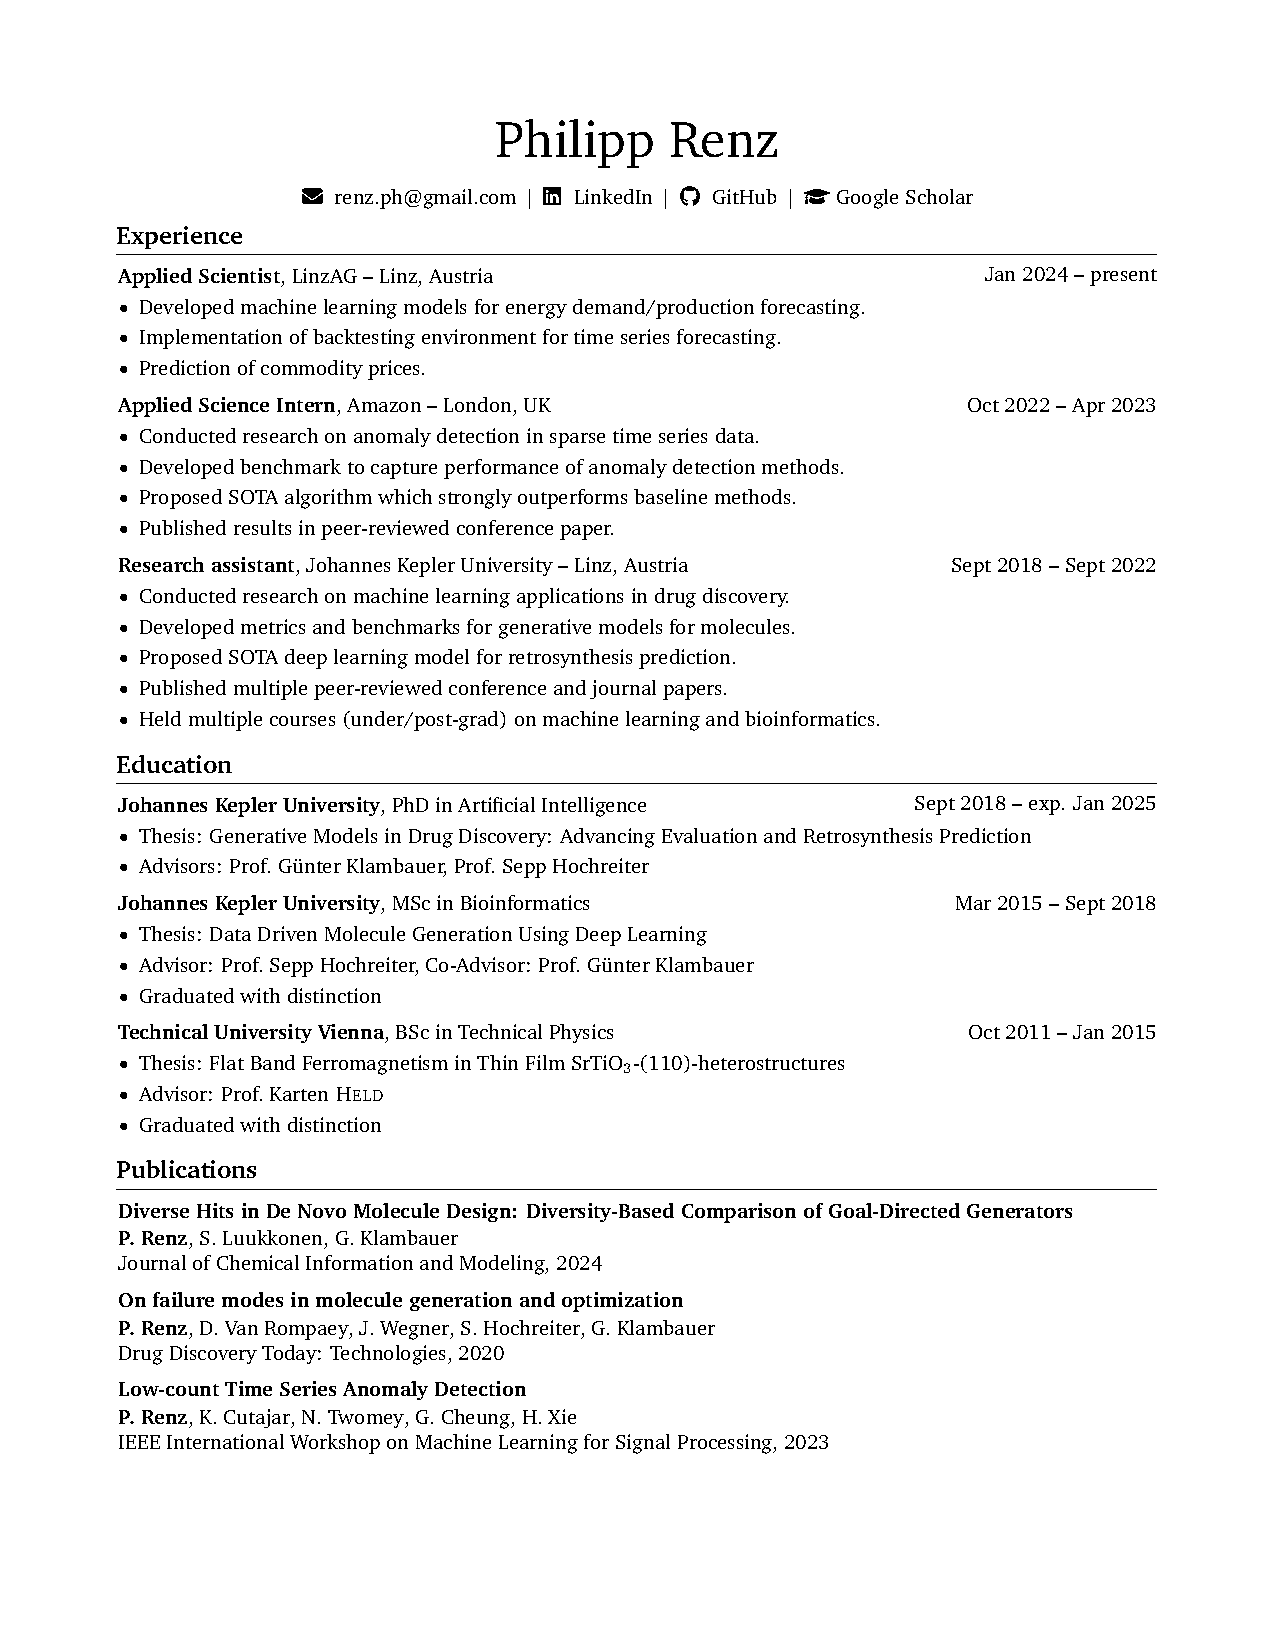
\includepdf[
    pages=-,
    frame,
    width=1.1\linewidth,
    pagecommand={\thispagestyle{scrheadings}},
    offset=0cm 0.9cm,
    trim=0.5cm 0.1cm 0.5cm 0.1cm,
]{CV_Philipp_Renz.pdf}
% \fi

%%%%%%%%%%%%%%%%%%%%%%%%%%%%
\printbibliography%

%%%%%%%%%
\appendix

\end{document}